% Options for packages loaded elsewhere
\PassOptionsToPackage{unicode}{hyperref}

% Set document class options
\documentclass[webpdf,large,modern,unnumsec,namedate]{oup-authoring-template}

% one column
\onecolumn

%\usepackage{showframe}

% line numbers
\usepackage{lineno}
\linenumbers

% use upquote if available, for straight quotes in verbatim environments
\IfFileExists{upquote.sty}{\usepackage{upquote}}{}

% From Pandoc template for its feature
\usepackage{xcolor}
\usepackage{hyperref}

\hypersetup{
  pdftitle={Does stomatal patterning in amphistomatous leaves minimize the CO\_2 diffusion path length within leaves?},
  pdfkeywords={amphistomy, Arabidopsis thaliana, CO\(_2\)
diffusion, finite element method, optimality, photosynthesis, stomata},
  breaklinks=true,
  bookmarks=true,
  hidelinks,
  pdfcreator={LaTeX via pandoc}}



% tightlist command for lists without linebreak
\providecommand{\tightlist}{%
  \setlength{\itemsep}{0pt}\setlength{\parskip}{0pt}}




% Counters for addresses and footnotes
\newcounter{correspcnt} % For author footnotes
\renewcommand*{\thecorrespcnt}{\fnsymbol{correspcnt}}
\newcounter{addrcnt} % For author addresses

% Macros for dealing with affiliations, footnotes, etc.
\makeatletter

\def\MyNewLabel#1#2#3{\expandafter\gdef\csname #1@#2\endcsname{#3}}

\def\MyRef#1#2{\@ifundefined{#1@#2}{???}{\csname #1@#2\endcsname}}

\newcommand*\ifcounter[1]{%
  \ifcsname c@#1\endcsname
    \expandafter\@firstoftwo
  \else
    \expandafter\@secondoftwo
  \fi
}

\newcommand*\addrlblbycode[1]{%
  \ifcounter{ADDRLBL@#1}
    {}
    {\refstepcounter{addrcnt}\newcounter{ADDRLBL@#1}\setcounter{ADDRLBL@#1}{\value{addrcnt}}}%
    \arabic{ADDRLBL@#1}%
}

\newcommand*\addrbycode[1]{%
  \ifcounter{ADDR@#1}
    {}
    {\newcounter{ADDR@#1}%
     \address[\addrlblbycode{#1}]{\MyRef{ADDRTXT}{#1}}}%
}

\newcommand*\corresplblbycode[1]{%
  \ifcounter{CORRESPLBL@#1}
    {}
    {\refstepcounter{correspcnt}\newcounter{CORRESPLBL@#1}\setcounter{CORRESPLBL@#1}{\value{correspcnt}}}%
    \fnsymbol{CORRESPLBL@#1}%
}

\newcommand*\correspbycode[1]{%
  \ifcounter{CORRESP@#1}
    {}
    {\newcounter{CORRESP@#1}%
     \corresp[\corresplblbycode{#1}]{\MyRef{CORRESPTXT}{#1}}}%
}

\makeatother

% Add missing \city command mentioned in documentation but absent from cls
\providecommand\city[1]{#1}

% Create labels for Addresses if the are given in Elsevier format
   \MyNewLabel{ADDRTXT}{UHM}{%
  School of Life Sciences, University of Hawaiʻi at Mānoa, Honolulu, HI
96822%
 }
   \MyNewLabel{ADDRTXT}{CU}{%
  Ecology and Evolutionary Biology, University of Colorado, Boulder, CO
80309%
 }
   \MyNewLabel{ADDRTXT}{NIAB}{%
  Department of Crop Science and Production Systems, NIAB, Cambridge,
CB3 0LE, UK%
 }
   \MyNewLabel{ADDRTXT}{UCD}{%
  Department of Plant Sciences, University of California, Davis, CA
95616%
 }
   \MyNewLabel{ADDRTXT}{UWM}{%
  Department of Botany, University of Wisconsin, Madison, WI 53706%
 }

% Create labels for Footnotes if they are given in Elsevier format

% Pandoc header-include feature
\usepackage{setspace}
\onehalfspacing
\usepackage[nomarkers,tablesfirst]{endfloat}
\usepackage{hyperref}
\renewcommand{\figureautorefname}{Fig.}
\usepackage[detect-none]{siunitx}
\sisetup{range-phrase = \text{--}}
\usepackage{caption}
\usepackage{newunicodechar,graphicx}
\DeclareRobustCommand{\okina}{\raisebox{\dimexpr\fontcharht\font`A-\height}{\scalebox{0.8}{`}}}
\newunicodechar{ʻ}{\okina}
% Pandoc header-include feature
\usepackage{booktabs}

\begin{document}

\journaltitle{Journal Title Here}
\DOI{DOI HERE}
\copyrightyear{YYYY}
\pubyear{YYYY}
\access{Advance Access Publication Date: Day Month Year}
\appnotes{Paper}

\firstpage{1}



\title[]{Does stomatal patterning in amphistomatous leaves minimize the
CO\(_2\) diffusion path length within leaves?}

\newcounter{thisauthcorresp} % For storage if author is corresponding author
\newcounter{thisauththanks} % For storage if author has thanks



\author[%
\addrlblbycode{UHM},\addrlblbycode{CU}%
,\refstepcounter{correspcnt}\setcounter{thisauthcorresp}{\value{correspcnt}}\fnsymbol{thisauthcorresp}%
%
%
]{Jacob L. Watts}

\addrbycode{UHM}
\addrbycode{CU}

\corresp[\fnsymbol{thisauthcorresp}]{Corresponding author. \href{mailto:Jacob.Watts-1@colorado.edu}{\nolinkurl{Jacob.Watts-1@colorado.edu}}}




\author[%
\addrlblbycode{NIAB}%
%
%
%
]{Graham J. Dow}

\addrbycode{NIAB}






\author[%
\addrlblbycode{UCD}%
%
%
%
]{Thomas N. Buckley}

\addrbycode{UCD}






\author[%
\addrlblbycode{UHM},\addrlblbycode{UWM}%
%
%
%
]{Christopher D. Muir}

\addrbycode{UHM}
\addrbycode{UWM}






% Add author mark
\authormark{Jacob L. Watts et al.}

\received{Date}{0}{Year}
\revised{Date}{0}{Year}
\accepted{Date}{0}{Year}

%\editor{Associate Editor: Name}

\abstract{
Photosynthesis is co-limited by multiple factors depending on the plant
and its environment. These include biochemical rate limitations,
internal and external water potentials, temperature, irradiance, and
carbon dioxide (CO\(_2\)). Amphistomatous leaves have stomata on both
abaxial and adaxial leaf surfaces. This feature is considered an
adaptation to alleviate CO\(_2\) diffusion limitations in productive
environments as the diffusion path length from stomate to chloroplast is
effectively halved in amphistomatous leaves. Plants may also reduce
CO\(_2\) limitations through other aspects of optimal stomatal anatomy:
stomatal density, distribution, patterning, and size. A number of
studies have demonstrated that stomata are overdispersed compared to a
random distribution on a single leaf surface; however, despite their
prevelance in nature and near ubiquity among crop species, much less is
known about stomatal anatomy in amphistomatous leaves, especially the
coordination between leaf surfaces. Here we use novel spatial statistics
based on simulations and photosynthesis modeling to test hypotheses
about how amphistomatous plants may optimize CO\(_2\) diffusion in the
model angiosperm \emph{Arabidopsis thaliana} grown in different light
environments. We find that 1) stomata are overdispersed, but not ideally
dispersed, on both leaf surfaces across all light treatments; 2) the
patterning of stomata on abaxial and adaxial leaf surfaces is
independent; and 3) the theoretical improvements to photosynthesis from
abaxial-adaxial stomatal coordination are miniscule (\(\ll 1\)\%) across
the range of feasible parameter space. However, we also find that 4)
stomatal size is correlated with the mesophyll volume that it supplies
with CO\(_2\), suggesting that plants may optimize CO\(_2\) diffusion
limitations through alternative pathways other than ideal, uniform
stomatal spacing. We discuss the developmental, physical, and
evolutionary constraits which may prohibit plants from reaching this
theoretical adaptive peak of uniform stomatal spacing and inter-surface
stomatal coordination. These findings contribute to our understanding of
variation in the anatomy of amphistomatous leaves.}

\keywords{amphistomy; Arabidopsis thaliana; CO\(_2\) diffusion; finite
element method; optimality; photosynthesis; stomata}


\maketitle


\section{Introduction}\label{introduction}

Stomatal anatomy (e.g.~size, density, distribution, and patterning) and
movement regulate gas exchange during photosynthesis, namely CO\(_2\)
assimilation and water loss through transpiration. Since waxy cuticles
are mostly impermeable to CO\(_2\) and H\(_2\)O, stomata are the primary
entry and exit points through which gas exchange occurs despite making
up a small percentage of the leaf area \citep{lange_responses_1971}.
Stomata consist of two guard cells which open and close upon changes in
turgor pressure or hormonal cues \citep{mcadam_linking_2016}. The
stomatal pore leads to an internal space known as the substomatal cavity
where gases contact the mesophyll. Once in the mesophyll, CO\(_2\)
diffuses throughout a network of intercellular air space (IAS) and into
mesophyll cells where CO\(_2\) assimilation (\(A\)) occurs within the
chloroplasts \citep{lee_diffusion_1964}. Stomatal conductance and
transpiration are determined by numerous environmental and anatomical
parameters such as vapor pressure deficit (VPD), irradiance,
temperature, wind speed, leaf water potential, IAS geometry, mesophyll
cell anatomy, and stomatal anatomy. The latter of these is the focus of
this study, with discussion of other interacting variables.

Many successful predictions about stomata and other C\(_3\) leaf traits
can be made by hypothesizing that natural selection should optimize
CO\(_2\) gain per unit of water loss for any given set of environmental
parameters, including their variability
\citep{cowan_stomatal_1977, buckley_optimal_2017, sperry_predicting_2017}.
Total stomatal area (size \(\times\) density) is optimized for
operational conductance (\(g_\text{s,op}\)) rather than maximum
conductance (\(g_\text{s,max}\)) such that stomatal apertures are most
responsive to changes in the environment at their operational aperture
\citep{franks_physiological_2012, liu_scaling_2021}. Stomatal aperture
can compensate for suboptimal stomatal densities to an extent
\citep{bussis_stomatal_2006}, but stomatal density and size ultimately
determine a leaf's theoretical \(g_\text{s,max}\)
\citep{sack_developmental_2016}, which is proportional to
\(g_\text{s,op}\) under typical conditions
\citep{mcelwain_using_2016, murray_consistent_2020}. Additionally, low
stomatal densities lead to irregular and insufficient CO\(_2\) supply
and reduced photosynthetic efficiency in leaf areas far from stomata
\citep{pieruschka_lateral_2006, morison_lateral_2005}, while high
stomatal densities can reduce water use efficiency (WUE)
\citep{bussis_stomatal_2006} and incur excessive metabolic costs
\citep{de_boer_optimal_2016, deans_optimization_2020}. Stomatal density
positively co-varies with irradiance during leaf development and
negatively co-varies with CO\(_2\) concentration
\citep{gay_influence_1975, schoch_dependence_1980, woodward_stomatal_1987, royer_stomatal_2001},
consistent with optimality predictions. In most species, stomata occur
only on the abaxial (usually lower) leaf surface; but amphistomy, the
occurrence of stomata on both abaxial and adaxial leaf surfaces, is also
prevalent in high light environments with constant or intermittent
access to sufficient water
\citep{mott_adaptive_1982, jordan_using_2014, muir_light_2018, drake_two_2019, muir_is_2019}.
Amphistomy effectively halves the CO\(_2\) diffusion path length and
boundary layer resistance by doubling boundary layer conductance \citep[
\citet{harrison_influence_2020}]{parkhurst_adaptive_1978, mott_amphistomy_1991}.
Ab- and adaxial leaf surfaces were found to function independent of one
another in wheat, an important crop, with the adaxial surface
demonstrating higher photosynthetic capacity \citep{wall_stomata_2022}.
These results highlight the utmost importance of amphistomy for some
plants.

Despite the success of optimality predictions, stomatal anatomy may be
partially constrained by physical and developmental limits on phenotypic
expression
\citep{croxdale_stomatal_2000, harrison_influence_2020, muir_how_2023}.
A number of physical and developmental processes constrain stomatal
anatomy trait space. For example, almost all stomata follow the one cell
spacing rule to maintain proper stomatal functioning as guard cell
movement requires the rapid exchange of ions with neighboring epidermal
cells (i.e.~subsidiary cells)
\citep{geisler_oriented_2000, dow_physiological_2014}. This would
prevent stomata from being strongly clustered; however, some species
(notably in \emph{Begonia}) appear to benefit from the overlapping vapor
shells caused by stomatal clustering in dry environments
\citep{yi_gan_stomatal_2010, lehmann_effects_2015, papanatsiou_stomatal_2017}.
Historically, stomatal patterning in eudicot angiosperms was thought to
be random with an exclusionary distance surrounding each stomate
\citep{sachs_developmental_1974}; however, the developmental controls of
stomatal patterning are more complex. \citet{croxdale_stomatal_2000}
reviews three developmental theories which attempt to explain stomatal
patterning in angiosperms: inhibition, cell lineage, and cell cycle,
ultimately arguing for a cell cycle based control of stomatal
patterning. \citet{pillitteri_mechanisms_2012} review the short and long
distance signalling pathways associated with stomatal spacing and
development, which include cell to cell communication and whole plant
integration to ensure the proper spacing of stomata across a single leaf
surface depending on environmental ques. Much less is known about the
development of stomata on the adaxial leaf surface in amphistomatous
plants. Stomatal size is additionally constrained by genome size with
larger genomes leading to larger minimum guard cell size
\citep{jordan_environmental_2015, roddy_scaling_2020}. Despite these
limitations, ecophysiological theory still predicts optimal stomatal
anatomy, the details of which are discussed below.

The patterning and spacing of stomata on the leaf affects photosynthesis
in C\(_3\) leaves by altering the CO\(_2\) diffusion path length from
stomata to sites of carboxylation in the mesophyll. Maximum
photosynthetic rate (\(A_\text{max}\)) in C\(_3\) plants is generally
co-limited by biochemistry and diffusion, but modulated by light
availability
\citep{parkhurst_intercellular_1990, manter_ci_2004, carriqui_diffusional_2015}.
Low light decreases CO\(_2\) demand by limiting electron transport rate,
leading to relatively high internal CO\(_2\) concentration
(\(C_\text{i}\)) and low \(A_\text{max}\) \citep{kaiser_metabolic_2016}.
In contrast, well hydrated leaves with open stomata in high light,
photosynthesis is often limited by CO\(_2\) supply as resistances from
the boundary layer, stomatal pore, sub-stomatal cavity, and mesophyll
can result in insufficient CO\(C_2\) supply at the chloroplast to
maximize photosynthesis
\citep{farquhar_biochemical_1980, lehmeier_cell_2017}. In this study, we
focus primarily on how stomatal patterning affects diffusion.

Assuming uniform mesophyll diffusion resistance in all directions
(homogenous porous medium), an ideal stomatal anatomy can be predicted.
To maximize CO\(_2\) supply from the stomatal pore to chloroplasts,
stomata should be uniformly distributed in an equilateral triangular
grid on the leaf surface so as to minimize stomatal number and CO\(_2\)
diffusion path length \citep{parkhurst_diffusion_1994}. An equilateral
triangular grid is ideal because it maximizes the average distance
between stomata, for a given stomatal density, and thereby minimizes the
average distance between any point in the mesophyll to its nearest
stomate. Assuming a homogenous mesophyll, this is the most efficient
pattern to supply CO\(_2\) to a leaf volume.

Such an assumption, though an oversimplification, is a powerful tool for
photosynthesis modelling, and may provide insight into how real leaves
diverge from this. In real leaves, as the diffusion rate of CO\(_2\)
though liquid is approximately \(10^4\times\) slower than CO\(_2\)
diffusion through air, mesophyll resistance is generally thought to be
primarily limited by liquid diffusion
\citep{aalto_three-dimensional_2002, evans_resistances_2009}, but
diffusion through the IAS has also been shown to be a rate limiting
process because the tortuous, disjunct nature of the IAS can greatly
increase diffusion path lengths \citep{harwood_understanding_2021}.
Additionally, tortuosity is higher in horizontal directions (parallel to
leaf surface) than vertical directions (perpendicular to leaf surface)
because of the cylindrical shape and vertical arrangement of palisade
mesophyll cells \citep{earles_beyond_2018, harwood_understanding_2021}.
However, the ratio of lateral to vertical diffusion rate is still
largely unknown and may be a highly variable trait in leaves
\citep{morison_lateral_2005, pieruschka_lateral_2005, pieruschka_lateral_2006, morison_does_2007}.
Depending on the thickness of the leaf, porosity of the leaf mesophyll,
tortuosity of the IAS, and lateral to vertical diffusion rate ratio,
minimizing diffusion path length for CO\(_2\) via optimally distributed
stomata may yield significant increases in CO\(_2\) supply for
photosynthesis and higher \(A_\text{max}\). Or plants may simply
coordinate the development of stomata and mesophyll IAS to reach another
optimal solution which does not rely on uniformly distributed stomata
\citep{baillie_developmental_2020}.

We hypothesized that, in the absence of any constraint and assuming
homogenous mesophyll diffusion resistance, natural selection will favor
stomatal patterning and distribution to minimize the diffusion path
length. In amphistomatous leaves, this would be accomplished by 1) a
uniform, equilateral triangular distribution of stomata on both abaxial
and adaxial leaf surfaces and 2) coordinated stomatal spacing on each
surface that offsets the position of stomata
(\autoref{fig:ideal-amphi-grid}). Coordination between leaf surfaces is
defined in this study as the occurrence of stomata in areas farthest
from stomata on the opposite leaf surface. Additionally, because
CO\(_2\) is more limiting for photosynthesis under high light, we
hypothesize that in high light 3) there should be more stomata, and 4)
stomata should be more overdispersed (closer to equilateral triangular
grid) compared to a random distribution than in low light. Finally,
since, in measures of whole leaves, stomatal area rather than stomatal
density is optimized for operational conductance, we hypothesize that 5)
stomatal length (and hence its area) will be positively correlated with
the area of the leaf surface to which it is spatial closest as defined
by Voronoi tessellation techniques. We refer to this as the `stomatal
zone', the leaf area surrounding a focal stomate closest to that stomate
and therefore the zone it supplies with CO\(_2\)). This way, each
stomate may be optimally sized relative to the mesophyll volume it
supplies. Hypothesis 3 is already well supported in many species
\citep{poorter_metaanalysis_2019}, but it is useful here to confirm that
light treatments induced plasticity in the expected direction.

\begin{figure}[ht]
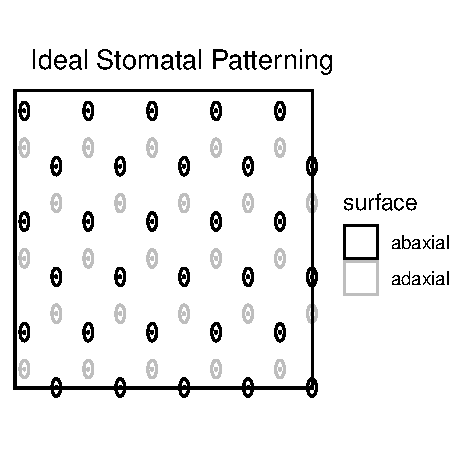
\includegraphics[width = 4in]{figures/ideal-amphi-grid.pdf}
\caption{Idealized amphistomatous stomatal grid with uniform stomatal patterning and perfect abaxial-adaxial coordination.}
\label{fig:ideal-amphi-grid}
\end{figure}

To test these hypotheses, we grew the model plant \emph{Arabidopsis
thaliana} in high, medium, and low light and measured stomatal density,
size, and patterning on both leaf surfaces, and spatial coordination
between them. We use Voronoi tessellation techniques to calculate
stomatal zones. We also used a 2-D porous medium approximation of
CO\(_2\) diffusion and photosynthesis to predict the photosynthetic
advantage of optimal versus suboptimal coordination in stomatal
coordination between surfaces. Specifically, we predicted that traits
which affect diffusion path length (leaf thickness, stomatal density,
leaf porosity), diffusion rate (determined by temperature, pressure),
and CO\(_2\) demand (Rubisco concentration, light) would modulate the
advantage of optimal stomatal arrangement following the relationships
outlined in \autoref{tab:hypotheses}. Here, we integrate over reasonable
parameter space to determine the ecophysiological context most likely to
favor stomatal coordination in amphistomatous leaves.

\begin{table}[ht]
\centering
\begin{tabular}{ll}
  \hline
trait & relationship \\ 
  \hline
leaf thickness & + \\ 
  interstomatal distance & + \\ 
  leaf porosity & - \\ 
  light & + \\ 
   \hline
\end{tabular}
\caption{A summary of the hypothesized relationships between leaf traits and environmental conditions and photosynthetic advantage of stomatal spatial coordination in amphistomatous leaves.} 
\label{tab:hypotheses}
\end{table}

\section{Materials and methods}\label{materials-and-methods}

\subsection{Data Preparation}\label{data-preparation}

Plant material, growth conditions, and three-dimensional confocal
imaging are described in \citet{dow_disruption_2017}. Briefly, Columbia
(Col-0) ecotype of \emph{Arabidopsis thaliana} (L.) Heynh. plants were
grown in three different light environments: low light (PAR = 50
\(\mu \text{mol}~\text{m}^{-2}~\text{s}^{-1}\)), medium light (100
\(\mu \text{mol}~\text{m}^{-2}~\text{s}^{-1}\)), and high light (200
\(\mu \text{mol}~\text{m}^{-2}~\text{s}^{-1}\)). PAR stands for
photosynthetically active radiation. \emph{A. thaliana} responds
strongly to light levels over this range
\citep{bailey_acclimation_2001}, though natural populations in open
canopies can experience
\(\text{PAR} > 800~\mu \text{mol}~\text{m}^{-2}~\text{s}^{-1}\)
\citep{callahan_shade-induced_2002}. Seeds were surface-sterilized and
stratified at 4 °C for 3--5 d in 0.15\% agarose solution and then sown
directly into Pro-Mix HP soil (Premier Horticulture; Quakerstown, PA,
USA) and supplemented with Scott's Osmocote Classic 14-14-14 fertilizer
(Scotts-Sierra, Marysville, OH, USA). At 10--14 d, seedlings were
thinned so only one seedling per container remained. Plants were grown
to maturity in growth chambers where the conditions were as follows: 16
: 8 h, 22 : 20°C, day : night cycle. Imaging of the epidermis and
internal leaf structures was performed using a Leica SP5 confocal
microscope (Leica Microsystems, Wetzlar, Germany) with the protocol
developed by \citet{wuyts_high-contrast_2010} with additional
modification described in \citet{dow_disruption_2017}. We captured 132
images in total, making 66 abaxial-adaxial image pairs. Images were
square with an area of 0.386 mm\(^2\). We measured stomatal position and
length using ImageJ \citep{schneider_nih_2012}. A number of synthetic
leaf surface data sets were also simulated (details below) to generate
null distributions against which to test our hypotheses and to avoid any
methodological influence on our results (e.g.~boundary effects when
calculating stomatal patterning). All synthetic leaf surfaces were
simulated based on the size of the real leaf images and stomatal
densities matched those of real leaf images.

\subsection{Single surface analyses}\label{single-surface-analyses}

We compared observed stomatal patterning to an ideal pattern (uniform
equilateral triangular grid) and a null model (random uniform
distribution). The terminology is unfortunately confusing because the
word `uniform' is used in different ways. A uniform equilateral
triangular grid means that the distance between stomata is uniform; a
random uniform distribution means that a stomate has an equal
probability (i.e.~uniform) of occurring anyone on the leaf surface. To
limit confusion, we refer to the ideal pattern as uniform (equilateral
triangle grid) and the null pattern as random (random uniform). When
observed stomatal patterns are more dispersed than expected under random
patterning, we refer to this as overdispersed. Note, however, that
overdispersed compared to random is still less dispersed than ideal,
because the ideal pattern is maximally dispersed.

We tested whether stomata overdispersed by comparing each observed, real
leaf stomatal pattern to an array of synthetic data simulated from a
random distribution. For each observed leaf surface image with \(n\)
stomata we generated \(10^3\) synthetic surfaces with \(n\) stomata
uniformly randomly distributed on the surface. For each sample image, we
compared the observed Nearest Neighbor Index (\(\mathrm{NNI}\)) to the
null distribution of \(\mathrm{NNI}\) values calculated from the
synthetic data set. \(\mathrm{NNI}\) is the ratio of observed mean
distance (\(\overline{D}_O\)) to the expected mean distance
(\(\overline{D}_E\)) where \(\overline{D}_E\) is:

\begin{equation}\label{eq:emd}
  \overline{D}_E = \frac{0.5}{\sqrt{A_\text{leaf} / n_\text{stomata}}}.
\end{equation}

\noindent \(A_\text{leaf}\) is leaf area visible in the sampled field
and \(n_\text{stomata}\) the number of stomata. \(\overline{D}_E\) is
the theoretical average distance to the nearest neighbor of each stomate
if stomata were uniformly randomly distributed
\citep{clark_distance_1954}. \(\overline{D}_O\) calculated for each
synthetic data set is:

\begin{equation}\label{eq:omd}
  \overline{D}_O = \frac{\sum_{i=1}^{n_\text{stomata}}d_i}{n_\text{stomata}},
\end{equation}

\noindent where \(d_i\) is the distance between \(\text{stomate}_i\) and
its nearest neighbor. We calculated \(\mathrm{NNI}\) using the \emph{R}
package \textbf{spatialEco} version 2.0.2 \citep{evans_spatialeco_2023}.
The observed stomatal distribution is overdispersed relative to a random
distribution if the observed \(NNI\) is greater than 95\% of the
synthetic \(\mathrm{NNI}\) values (one-tailed test). We adjusted
\(P\)-values to account for multiple comparisons using the
Benjamini-Hochberg \citep{benjamini_controlling_1995} false discovery
rate procedure implemented in the \emph{R} package \textbf{multtest}
version 2.56.0 \citep{wong_multiple_2005}.

For each sample image, we also simulated \(10^3\) synthetic leaf
surfaces with \(n\) stomata ideally, uniformly dispersed in an
equilateral triangular grid. To account for uncertainty in the stomatal
density of each sample image with \(n\) stomata, we integrated over
plausible stomatal densities and then conditioned on synthetic leaf
surfaces with exactly \(n\) stomata. The simulated stomatal count was
drawn from a Poisson distribution with the mean parameter \(\lambda\)
drawn from a Gamma distribution with shape \(n\) and scale 1
(\(\lambda \sim \Gamma(n, 1)\)). \(\Gamma(n, 1)\) is the posterior
distribution of \(\lambda\) with a flat prior distribution. This
integration was necessary to remove any artifacts of uncertainty in the
true stomatal density of the sample leaves.

We developed a dispersion index \(\mathrm{DI}\) to quantify how close
observed stomatal patterning is to random versus ideally patterned in an
equilateral triangular grid. \(\mathrm{DI}\) varies from zero to one,
where zero is random and one is ideally patterned:

\begin{equation}\label{eq:disp}
  \mathrm{DI} = \frac{\mathrm{NNI} - \text{median}(\mathrm{NNI_{random}})}{\text{median}(\mathrm{NNI_{ideal}}) - \text{median}(\mathrm{NNI_{random}})}
\end{equation}

\noindent \(\mathrm{NNI}\) is calculated for each sample image as
described above; \(\text{median}(\mathrm{NNI_{random}})\) and
\(\text{median}(\mathrm{NNI_{uniform}})\) are calculated from the
synthetic data specific to each sample image as described above. We
tested whether light treatment affects \(\mathrm{DI}\) and stomatal
density (\(D_S\)) using analysis of variance (ANOVA).

Finally, we examined the relationship between stomatal zone area and
stomatal length using a Bayesian linear mixed-effects model fit with the
\emph{R} package \textbf{brms} version 2.20.4
\citep{burkner_brms_2017, burkner_advanced_2018} and \emph{Stan} version
2.33.1 \citep{stan_development_team_stan_2023}. Stomatal zone area was
calculated using Voronoi tessellation
(e.g.~\autoref{fig:tessellation-example}). The stomatal zone area,
\(S_\text{area}\), is the region of the leaf surface whose distance to
stomate, \(S\), is less than the distance to any other stomate, \(S\).
Stomatal length was measured in ImageJ \citep{schneider_nih_2012}. We
modeled fixed effects of surface, light treatment, stomatal length, and
their 2- and 3-way interactions on \(\sqrt{S_\text{area}}\). We included
random intercepts, random effects of surface, random slopes, and random
surface-by-slope interactions within both plant and individual to
account for nonindependence of stomata within the same plant or
individual. We also modeled residual variance as a function of light
treatment. We sampled the posterior distribution from 4 chains with 1000
iterations each after 1000 warmup iterations. We calculated convergence
diagnostics (\(\hat{R}\)) and effective sample sizes following
\citet{vehtari_rank-normalization_2021}. We estimated the marginal slope
and 95\% highest posterior density (HPD) intervals between stomatal
length and \(\sqrt{S_\text{area}}\) using the \emph{emtrends} function
in the \emph{R} package \textbf{emmeans} version 1.9.0
\citep{lenth_emmeans_2023}.

\begin{figure}[ht]
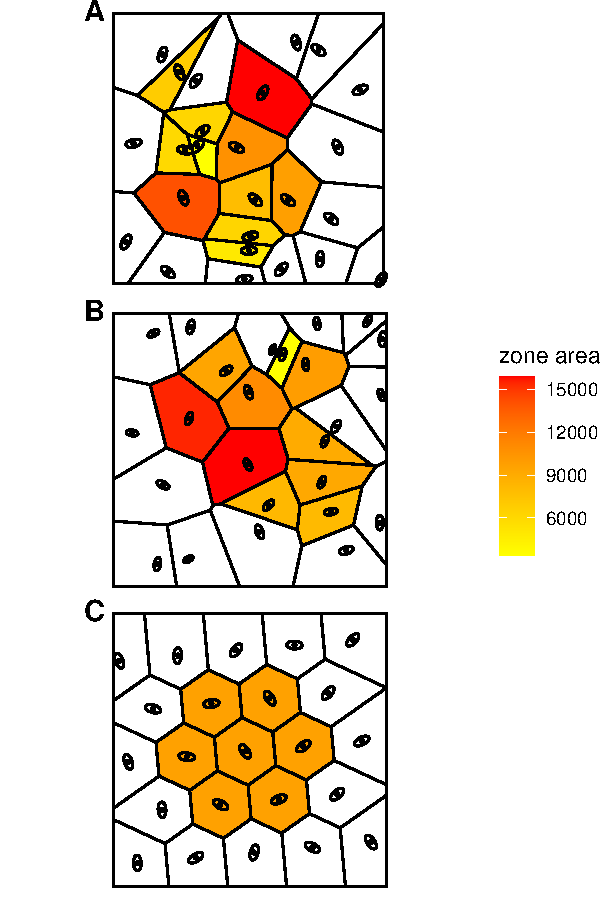
\includegraphics[height = \textheight]{figures/tessellation-example.pdf}
\caption{Examples of synthetic and real leaf surfaces.  A) Uniform random synthetic leaf surface; B) Example of real leaf surface; C) Uniformly distributed synthetic leaf surface. The zone defined by each stomate was calculated with voronoi tessellation and correlated with stomatal length in real leaves.}
\label{fig:tessellation-example}
\end{figure}

\subsection{Paired Abaxial and Adaxial Surface
Analysis}\label{paired-abaxial-and-adaxial-surface-analysis}

To test whether the position of ab- and adaxial stomata are coordinated
we compared the observed distribution to a null distribution where the
positions on each surface are random. For each pair of surfaces
(observed or synthetic) we calculated the distance squared between each
pixel of the surface to the nearest stomatal centroid with the \emph{R}
package \textbf{raster} version 3.6.26 \citep{hijmans_raster_2023}. We
refer to this as the `nearest stomatal distance' or NSD. Then we
calculated the pixel-wise Pearson correlation coefficient. If stomatal
positions on each surface are coordinated to minimize the distance
between mesophyll and the nearest stomate, then we expect a negative
correlation. A pixel that is far from a stomate on one surface should be
near a stomate on the other surface (\autoref{fig:ideal-amphi-grid}). We
generated a null distribution of the correlation coefficient by
simulating \(10^3\) synthetic data sets for each observed pair. For each
synthetic data set, we simulated stomatal position using a random
uniform distribution, as described above, matching the number of stomata
on abaxial and adaxial leaf surfaces to the observed data. Stomatal
positions on each surface are coordinated if the correlation coefficient
of the NSD between observed ab- and adaxial surfaces is greater than
95\% of the synthetic correlation values (one-tailed test).

\subsection{Modeling Photosynthesis}\label{modeling-photosynthesis}

We modeled photosynthesis CO\(_2\) assimilation rate using a
spatially-explicit two-dimensional reaction diffusion model using a
porous medium approximation \citep{parkhurst_diffusion_1994} using the
finite element method (FEM) following \citet{earles_excess_2017}.
Consider a two-dimensional leaf where stomata occur on each surface in a
regular sequence with interstomatal distance \(U\). The main outcome we
assessed is the advantage of offsetting the position of stomata on each
surface compared to having stomata on the same \(x\) position on each
surface. With these assumptions, by symmetry, we only need to model two
stomata, one abaxial and one adaxial, from \(x = 0\) to \(x = U/2\) and
from the adaxial surface at \(y = 0\) to the abaxial surface at
\(y = L\), the leaf thickness. We arbitrarily set the adaxial stomate at
\(x = 0\) and toggled the abaxial stomata position between \(x = U/2\)
(offset) or \(x = 0\) (below adaxial stomate). The `coordination
advantage' of offset stomatal position on each surface is the
photosynthetic rate of the leaf with offset stomata compared to that
with stomata aligned in the same \(x\) position:

\begin{equation} \label{eq:coordination_advantage}
  \text{coordination advantage} = \frac{A_\text{offset}}{A_\text{aligned}}
\end{equation}

We modeled the coordination advantage over a range of leaf thicknesses,
stomatal densities, photosynthetic capacities, and light environments to
understand when offsetting stomatal position on each surface might
deliver a significant photosynthetic advantage
(\autoref{tab:model_var}). The complete model description is available
in the Supporting Information.

\begin{table}

\caption{\label{tab:model_var}The parameter range of model variables tested for their effect on coordination advantage (\autoref{eq:coordination_advantage}) using a 2-D porous medium approximation. We used regularly spaced values within each range and simulated across all combinations. Here we converted model units to more conventional units (e.g. m to $\mu$m). $I_0$: PPFD incident on the leaf surface; $\varphi_\text{pal}$: Fraction of intercellular airspace (aka porosity), palisade; $T_\text{leaf}$: Leaf thickness; $U$: Interstomatal distance}
\centering
\begin{tabular}[t]{lll}
\toprule
Variable & Parameter range & Units\\
\midrule
$I_0$ & $50-1000$ & $\mu$mol m$^{-2}$ s$^{-1}$\\
$\varphi_\text{pal}$ & $0.1-0.3$ & m$^3$ airspace m$^{-3}$ leaf\\
$T_\text{leaf}$ & $101-501$ & $\mu$m\\
$U$ & $17-169$ & $\mu$m\\
\bottomrule
\end{tabular}
\end{table}

\section{Results}\label{results}

Stomatal density of \emph{Arabidopsis thaliana} varies among light
treatments (ANOVA, \(F_{2,126} = 681, P = 2.88 \times 10^{-68}\))
because the density is much greater in the high light treatment
(\autoref{fig:density}). Density is consistently greater on abaxial leaf
surfaces across all light treatments (ANOVA,
\(F_{1,126} = 44.2, P = 8.21 \times 10^{-10}\); \autoref{fig:density}).
There is no evidence for an interaction between light treatment and
surface (ANOVA, \(F_{2,126} = 2.75 \times 10^{-2}, P = 0.973\)). Leaves
are amphistomatous with a mean stomatal density ratio of 0.44.

\begin{figure}[ht]
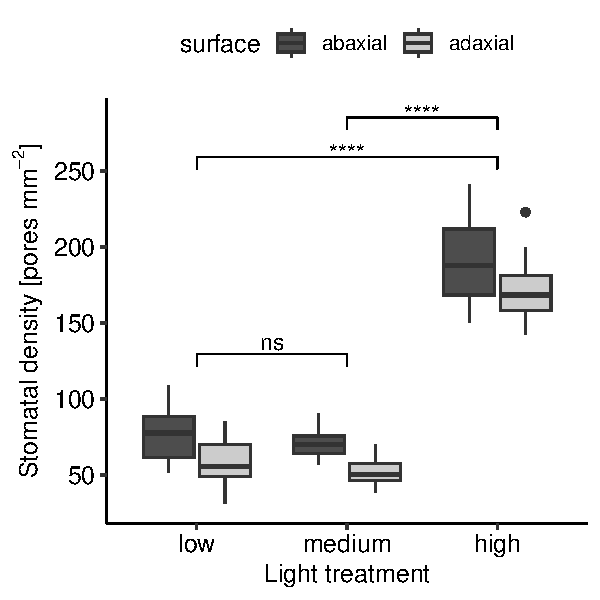
\includegraphics[width = 4in]{figures/density.pdf}
\caption{Stomatal density is higher in \textit{A. thaliana} plants grown under high light conditions. We determined statistical significance between light treatments using Tukey post-hoc tests. $^*~0.05 > P \ge 0.01; ^{**}~0.01 > P \ge 0.001; ^{***}~0.0001 > P \ge 0.0001; ^{***}~ P <0.0001$.}
\label{fig:density}
\end{figure}

\subsection{Stomatal patterning is non-random, but far from
uniform}\label{stomatal-patterning-is-non-random-but-far-from-uniform}

Many leaf surfaces (37 of 132, 28\%) are significantly overdispersed
compared to a random uniform distribution, but none were close to an
ideal, uniform equilateral triangular pattern (dispersion index = 1;
\autoref{fig:single-surface}). Before controlling for multiple
comparisons, 43.2\% are significantly overdispersed. The dispersion
index differs significantly among light treatments (ANOVA,
\(F_{2,126} = 8.55, P = 3.30 \times 10^{-4}\)) because the medium light
treatment is significantly less than the low treatment
(\autoref{fig:single-surface}). Dispersion index is consistently greater
on adaxial leaf surfaces across all light treatments (ANOVA,
\(F_{1,126} = 28.8, P = 3.67 \times 10^{-7}\);
\autoref{fig:single-surface}). There is no evidence for an interaction
between light treatment and surface (ANOVA,
\(F_{2,126} = 0.577, P = 0.563\)).

\begin{figure}[ht]
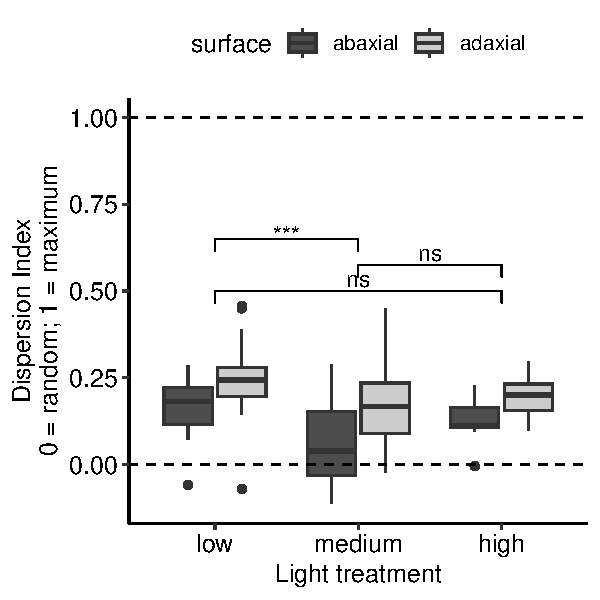
\includegraphics[width=4in]{figures/single-surface.pdf}
\caption{Stomata are more dispersed than expected under the null model of random patterning (dispersion index = 0) but far from a distribution that maximizes distance between stomata (dispersion index = 1; uniform patterning). We determined statistical significance between light treatments using Tukey post-hoc tests. $^*~0.05 > P \ge 0.01; ^{**}~0.01 > P \ge 0.001; ^{***}~0.0001 > P \ge 0.0001; ^{***}~ P <0.0001$.}
\label{fig:single-surface}
\end{figure}

\subsection{No evidence for coordinated stomatal position between
surfaces}\label{no-evidence-for-coordinated-stomatal-position-between-surfaces}

There is no evidence of spatial coordination between abaxial and adaxial
leaf surfaces. The pixel-wise correlation between nearest stomatal
distance (NSD) squared on paired abaxial and adaxial leaf surfaces is
not significantly less than zero in any of the 66 leaves
(\autoref{fig:dual-surface}). Before controlling for multiple
comparisons, 3\% are significantly \emph{positively} correlated. The NSD
correlation is not different among light treatments (ANOVA,
\(F_{2,63} = 2.28, P = 0.111\); \autoref{fig:dual-surface}).

\begin{figure}[ht]
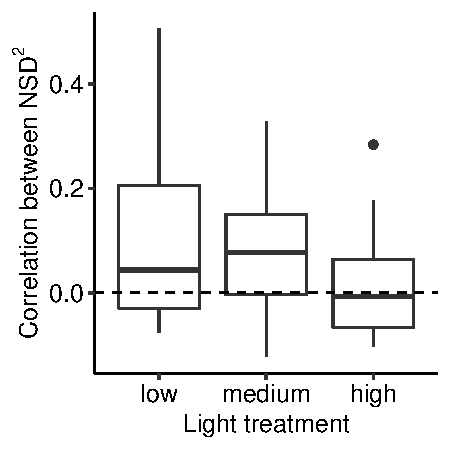
\includegraphics[width = 4in]{figures/dual-surface.pdf}
\caption{Pixel-wise correlation between near stomatal distance (NSD) squared on paired abaxial and adaxial leaf surfaces. Dashed line indicates zero correlation. Weak positive correlations are not significantly different from zero after correcting for multiple comparisons. The correlation does not differ among light treatments.}
\label{fig:dual-surface}
\end{figure}

\subsection{Larger stomata supply larger mesophyll
volumes}\label{larger-stomata-supply-larger-mesophyll-volumes}

All parameters in the Bayesian linear mixed-effects model converged
(\(\hat{R} < 1.01\)) and effective sample sizes exceeded \(10^3\).
Across all light treatments and leaf surfaces, stomatal length and
stomatal area are weakly positively correlated
(\autoref{fig:length-area}). The slope was significantly greater than
zero for all abaxial surfaces, but not for the adaxial surface in low
and medium light treatments. The estimated marginal slopes and 95\% HPD
intervals for each combination of light and surface is: low light,
abaxial surface: 1.928 {[}\numrange{0.779}{3.133}{]}; low light, adaxial
surface: 1.745 {[}\numrange{-0.041}{3.373}{]}; medium light, abaxial
surface: 1.085 {[}\numrange{0.328}{1.957}{]}; medium light, adaxial
surface: 0.656 {[}\numrange{-0.399}{1.691}{]}; high light, abaxial
surface: 0.597 {[}\numrange{0.316}{0.911}{]}; high light, adaxial
surface: 1.269 {[}\numrange{0.831}{1.721}{]}.

\begin{figure}[ht]
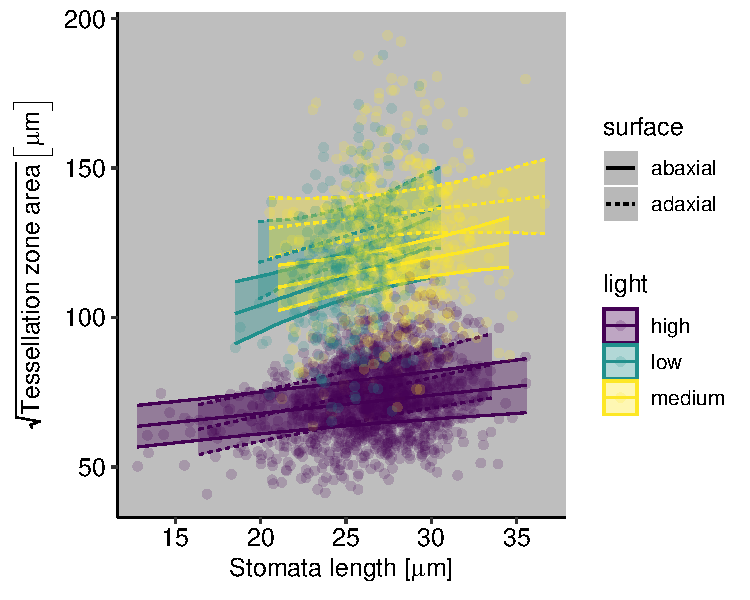
\includegraphics[width = 4in]{figures/length-area.pdf}
\caption{Stomatal length and stomatal zone area are positively correlated. Linear regression lines and 95\% confidence ribbons are from a Bayesian linear mixed-effects model.}
\label{fig:length-area}
\end{figure}

\subsection{Little benefit of coordinated stomatal
arrangement}\label{little-benefit-of-coordinated-stomatal-arrangement}

We used the finite element method (FEM) to model CO\(_2\) diffusion
within the leaf and photosynthesis as a 2-D porous medium. Across all
realistic parts of parameter space, the coordination advantage is much
less than 0.01 (\autoref{fig:model_summary}). For reference, a
log-response of ratio is 0.01 is approximately 1\%. The only exception
was for thin leaves (\(T_\text{leaf} = 100~\mu \text{m}\)) with few
stomata (\(U = 338~\mu \text{m}\), which corresponds to a stomatal
density of \(\approx 10~\text{mm}^{-2}\)), where lateral diffusion is
major constraint on CO\(_2\) supply. However, such thin leaves with so
few stomata are uncommon among C\(_3\) plants (some CAM plants have low
stomatal density \citep{males_stomatal_2017}). In other areas of
parameter space, lateral diffusion limitations were small relative to
those along the ab-adaxial axis (see Fig. S1 for a representative model
solution).

\begin{figure}[ht]
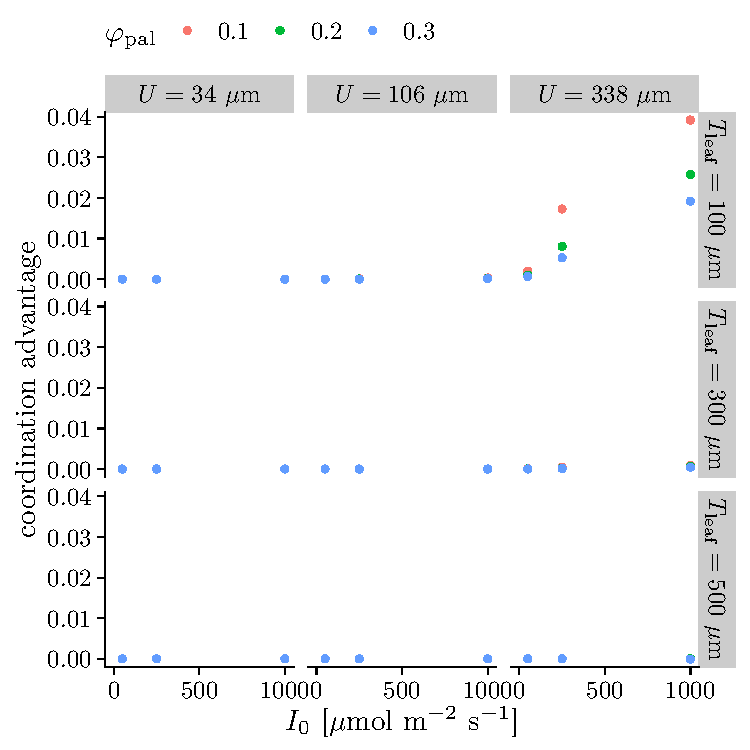
\includegraphics[width = 5in]{figures/model_summary.pdf}
\caption{There is little photosynthetic benefit of offsetting stomatal position each surface based on a 2-D model of photosynthesis. The coordination advantage (\autoref{eq:coordination_advantage}) is close to zero under nearly all of the parameter space \autoref{tab:model_var}, meaning that the photosynthetic rate of amphistomatous leaves with stomata optimally offset is nearly equal to leaves with stomata on each surface in the same position along the leaf plane. $I_0$: PPFD incident on the leaf surface; $\varphi_\text{pal}$: Fraction of intercellular airspace (aka porosity), palisade; $T_\text{leaf}$: Leaf thickness; $U$: Interstomatal distance.}
\label{fig:model_summary}
\end{figure}

\section{Discussion}\label{discussion}

Stomata cost resources to maintain \citep{deans_optimization_2020} and
expose leaves to risks such as hydraulic failure
\citep{wang_theoretical_2020} or infection by plant pathogens
\citep{melotto_stomatal_2017}. Therefore leaves should develop enough
stomata to adequately supply CO\(_2\) to chloroplasts, but not
overinvest. A widespread hypothesis in plant ecophysiology is that
natural selection optimizes traits like stomatal size, density, and
distribution to maximize carbon gain relative to any costs in a given
environmental context. In principle, spacing stomata to minimize the
average distance between stomatal pores and chloroplasts within the
mesophyll should increase carbon gain, all else being equal. However,
reducing this distance to its absolute minimum may be constrained by
developmental processes or the photosynthetic benefit may be too small
to be `seen' by natural selection (i.e.~the selection coefficient is
less than drift barrier \emph{sensu} \citet{sung_drift-barrier_2012}).
We also consider that our definition of optimal may be incorrect because
it is based on overly simplistic assumptions about leaf mesophyll
structure.

We tested five related hypotheses about stomatal spacing in
amphistomatous leaves using the model angiosperm \emph{Arabidopsis
thaliana} grown under different light intensities. First, we predicted
that stomata on each surface are overdispersed relative to a random
distribution, which should increase CO\(_2\) supply. Stomata on each
surface are overdispersed (\autoref{fig:single-surface}), but are not
ideally, uniformly patterned in an equilateral triangular grid as would
be optimal to minimize CO\(_2\) diffusion path length and equalize the
area supplied by each stomate (\autoref{fig:tessellation-example}).
Second, we predicted that an optimal amphistomatous leaf has offset
stomata such that stomata are more likely to appear on one leaf surface
if there is not a stomata directly opposite it on the other surface as
shown in \autoref{fig:ideal-amphi-grid}. However, there is no evidence
for coordination and the positions on each surface appear independent,
regardless of light treatment (\autoref{fig:dual-surface}). Third, we
predicted that plants respond plastically to higher light intensity by
increasing stomatal density. \emph{Arabidopsis} plants grown under high
light had higher stomatal density than the same genotype grown under low
and medium light intensity (\autoref{fig:density}). However, we found no
support for our fourth prediction that stomatal patterning would be
overdispersed at high light intensity (\autoref{fig:single-surface}).
Finally, we predicted that within leaf variation in stomatal size would
correlate with stomatal spacing, as larger stomata can supply larger
volumes of adjacent mesophyll. In all three light treatments, stomatal
size positively co-varied with the stomatal zone, i.e.~adjacent region
of mesophyll that would be supplied by that stomate
(\autoref{fig:length-area}).

Stomatal spacing on \emph{A. thaliana} leaves partially supports our
overall hypothesis that natural selection minimizes the average distance
between stomata and chloroplasts, for a given overall stomatal density.
There are three non-mutually exclusive hypotheses for why several of our
predictions were wrong. First, our predictions must be wrong because
they are based on overly simplistic assumption of a homogenous porous
medium within the mesophyll. Real leaf mesophylls are spatially
heterogenous and chloroplasts are distributed as discrete nodes. The
intercellular air space conductance is determined by its porosity and
tortuosity, both of which are heterogenous within the leaf. The palisade
is typically less porous than the spongy mesophyll (e.g.
\citet{therouxrancourt_bias_2017}), which should impact the optimal
patterning on stomata on ab- versus adaxial surfaces. Tortuosity is also
systematically greater in the palisade in the lateral direction parallel
to the leaf plane \citep{harwood_understanding_2021}. We might predict a
greater coordination advantage of offset stomata by accounting for
greater lateral tortuosity, but it is likely that benefit is still very
small under realistic parameter space. Quantifying the patterns of
heterogeneity in porosity, tortuosity, and other factors
\citep{earles_beyond_2018} using 3D imaging (e.g.
\citet{borsuk_structural_2022}) will be needed to generate more
realistic hypotheses about optimal stomatal spacing.

Second, spatio-temporal variation of internal conditions within leaves
and between stomatal responses may make uniform, coordinated stomatal
surfaces less beneficial
\citep{weyers_heterogeneity_1997, lawson_nature_1998, lawson_spatial_1999}.
This is because our model assumes a uniform leaf, the internal
conditions of which are periodic and solved empirically and therefore
stable. Any horizontal concentration gradients due to environmental
heterogeneity and variable induction times for interacting leaf
processes may reduce the benefit of uniform stomatal patterning. Third,
natural selection may be constrained by developmental processes that
prevent phenotypes from reaching their adaptive optima. Stomatal
development must be plastic to environmental cues interpreted through
long distance and cell-to-cell signalling pathways
\citep{pillitteri_mechanisms_2012}. This plasticity may come with the
cost of being unable to orchestrate the development of an absolutely
uniform stomatal grid. Fourth, the benefit of some traits may be of too
little consequence to result in fitness differences large enough to
respond to selection. We consider the plausibility of these alternative
hypotheses below and present ideas for future work to test them.

We assume an idealized leaf epidermal and mesophyll structure that is
homogenous and unconstrained by other tradeoffs. Real leaves not only
provide pathways for CO\(_2\) diffusion, but must supply water,
intercept light, and deter herbivores and pathogens. All of these
competing processes also happen on different time scales, and can be
observed as heterogeneity in stomatal density, aperture, and internal
leaf conditions across the leaf at any given moment
\citep{lawson_nature_1998, lawson_spatial_1999}. These competing
interests result in heterogeneous epidermal and mesophyll structure that
could alter predictions about optimal stomatal spacing. In order to
maintain consistent leaf water potential across the lamina, stomatal
density must be coordinated with vein density
\citep{fiorin_transport_2016}. Thus, stomatal spacing may be optimized
not at the interstomatal level, but at a higher level, coordinating
water transport and water loss. For example, the palisade mesophyll is
more tightly packed than the spongy mesophyll as an adaptation to
intercept light efficiently, so lateral diffusion may be more limiting
in the adaxial portion of the leaf. This may explain why adaxial leaf
surfaces have consistently higher dispersion indices than abaxial
surfaces across all light treatments (\autoref{fig:single-surface}).
Future gas exchange models should incorporate heterogenous mesophyll
structure and hydraulic traits such as veins.

We are not aware of a developmental pathway that ensures an idealized
placement of stomata on the leaf surface. Rather, stomatal development
is a dynamic process that must be plastic to environmental cues. Leaves
develop based on short and long distance signalling pathways which relay
information about incoming light, humidity, temperature, and surrounding
stomata to developing leaf tissues \citep{pillitteri_mechanisms_2012}.
Our results showing an intermediate level of dispersion in stomatal
spacing may be best explained by these developmental pathways which
ensure the proper spacing of stomata, with an added random effect
brought about by the necessity for plasticity in stomatal development
(\autoref{fig:single-surface}). However, deviations from ideal stomatal
spacing may compensated for by simultaneous and coordinated development
of the IAS \citep{baillie_developmental_2020}. The fact that stomata
which supply a greater mesophyll volume tend to be larger suggests that
plants may use coordinated development of multiple leaf anatomical
features to compensate for nonideal stomatal spacing
(\autoref{fig:length-area}).

In amphistomatous leaves, ideal stomatal spacing is complicated by a
third dimension. Our gas exchange model demonstrates little
photosynthetic gain from abaxial-adaxial stomatal coordination
(\autoref{fig:model_summary}). Even though lateral diffusion may limit
photosynthesis \citep{morison_lateral_2005}, the marginal gain from
optimally offsetting stomata is not sufficient to generate fitness
differences relative to the strength of genetic drift (i.e.~the
drift-barrier). We can similarly extrapolate that an ideal, equilateral
triangular stomatal spacing is only slightly better than a suboptimal
pattern. Any benefit garnered by ideal stomatal spacing may be
additionally offset by a cost to developmental flexibility in variable
environments
\citep{pillitteri_mechanisms_2012, baillie_developmental_2020}.
Explaining these observations as the result of weak selection is in
tension with the finding that stomatal size and zone positively covary,
which would suggest that small changes in lateral diffusion distance are
significant. As described above, the positive correlation between
stomatal size and zone may be explained by common developmental
processes rather than as an adaptation to maximize CO\(_2\) diffusion.
In any case, there is no evidence for coordinated development of both
leaf surfaces, and very little theoretical benefit to photosynthesis,
except in marginal circumstances which are exceptionally rare in nature.

Our study corroborates previous studies which demonstrate that stomata
are non-randomly distributed along the leaf surface as a result of
developmental mechanisms such as spatially biased arrest of stomatal
initials \citep{boetsch_arrest_1995}, oriented asymmetric cell division
\citep{geisler_oriented_2000}, and cell cycle controls
\citep{croxdale_stomatal_2000}. We do not investigate the potential
developmental pathways that influence stomatal dispersion in this study;
however, they are important to consider as these pathways could limit
plants from reaching a theoretical peak in the adaptive landscape:
uniform stomatal patterning. Instead, as this study suggests, plants may
simply compensate with higher stomatal density and by modulating
stomatal size to the area that they supply with CO\(_2\). To understand
why stomata are not ideally dispersed, more modeling (with more
realistic assumptions including vein density and IAS structure) should
be done to estimate the photosynthetic properties of varying stomatal
patterning. Additionally, genetic manipulation studies should attempt to
create mutants with clustered and uniformly patterned stomata for a
comparison of their photosynthetic traits. This could have important
implications for maximizing assimilation rates in crops as most crop
species are grown in high light where CO\(_2\) is often limiting. In
drought-prone environments, increased stomatal dispersion may increase
water use efficiency by reducing the number of stomata needed to achieve
the same internal CO\(_2\) concentration, \(C_\text{i}\). However, it
would be necessary to account for many other differences between
\emph{A. thaliana} and crop leaves and canopies.

Our results suggest that after optimizing stomatal density and having
developmental rules for spacing stomata relatively evenly, there may be
limited gains to further optimization. Therefore, developmental
constraints may be necessary to make sense of some features of stomatal
spacing and distribution. The possibility that ideal stomatal spacing is
not the ``tallest'' fitness peak must also be explored, as stomate size
is demonstrated in this study to covary with mesophyll volume supplied
with CO\(_2\). This may be especially true in highly variable
environments or in large tree species with sun and shade leaves where
developmental cues may change rapidly. The temporal component, not
considered here, could also have significant implications, as CO\(_2\)
may only be limiting to photosynthesis during short, relatively rare
periods when all other conditions are ideal. In these cases, the
theoretical benefits of ideal stomatal spacing are further diminished.
Future exploration of these competing hypotheses would require more
advanced modeling, additional exploration of IAS space development and
its effects on gas exchange, both real and modeled, and knowledge about
how often the species of interest is CO\(_2\) limited across of range of
natural settings. Despite these additional considerations, this study
represents an important contribution to understanding the potential
drivers of and limitations to stomatal anatomy in amphistomatous plants.

\section{Competing interests}

The authors declare no competing interests.

\section{Author contributions statement}

JLW and CDM conceived of the project, analyzed data, and wrote the
manuscript. GJD provided data. TNB contributed to model development and
helped edit the manuscript.


\renewcommand\refname{References}

\bibliographystyle{abbrvnat}
\bibliography{stomata-spacing.bib}

%% Author bio-pics with images


\end{document}
